\documentclass[border=3mm]{standalone}

\usepackage{tikz}
\usetikzlibrary{decorations.markings,arrows.meta}

\begin{document}

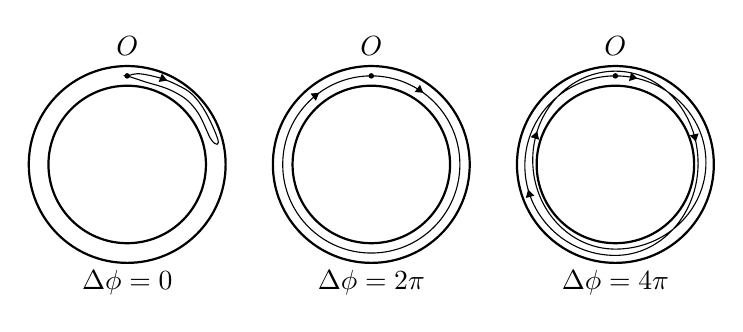
\begin{tikzpicture}

%% Middle Circle
\draw[thick] (0,0) circle (1cm);
\draw[thick] (0,0) circle (1.25cm);
\coordinate (1) at (0,1.125);
\draw[decoration={markings,mark=at position 0.1 with {\arrow{Triangle[scale=0.75]}},mark=at position 0.9 with {\arrow{Triangle[scale=0.75]}}},postaction={decorate}] (1) arc (90:-270:1.125cm);
\fill (1) circle (1pt);
\node at (0,1.5) {$O$};
\node at (0,-1.5) {$\Delta\phi=2\pi$};

%% Left Circle
\draw[thick] (-3.1,0) circle (1cm);
\draw[thick] (-3.1,0) circle (1.25cm);
\coordinate (2) at (-3.1,1.125);
\draw[decoration={markings,mark=at position 0.1 with {\arrow{Triangle[scale=0.75]}}},postaction={decorate}]  plot[smooth cycle, tension=.7] coordinates {(2) (-2.9,1.1469) (-2.5,1.0268) (-2.1933,0.8) (-1.9531,0.332) (-2.0263,0.3057) (-2.2268,0.6933) (-2.5,0.9201) (-2.9067,1.0603) (2)};
\fill (2) circle (1pt);
\node at (-3.1,1.5) {$O$};
\node at (-3.1,-1.5) {$\Delta\phi=0$};

%% Right Circle
\draw[thick] (3.1,0) circle (1cm);
\draw[thick] (3.1,0) circle (1.25cm);
\coordinate (3) at (3.1,1.125);
\draw[
	decoration={
		markings,
		mark=at position 0.02 with {\arrow{Triangle[scale=0.75]}},
		mark=at position 0.4 with {\arrow{Triangle[scale=0.75]}},
		mark=at position 0.6 with {\arrow{Triangle[scale=0.75]}},
		mark=at position 0.85 with {\arrow{Triangle[scale=0.75]}}
	},
	postaction={decorate}
] (3) arc (90:-90:1.15cm and 1.1cm) arc (270:90:1.05cm and 1.13cm) arc (90:-90:1.05cm and 1.17cm) arc (270:90:1.15cm and 1.14cm);
\fill (3) circle (1pt);
\node at (3.1,1.5) {$O$};
\node at (3.1,-1.5) {$\Delta\phi=4\pi$};
\end{tikzpicture}

\end{document}
